\documentclass[journal,10pt]{IEEEtran}
\usepackage{amsmath,amssymb,graphicx,booktabs,cite,url}
\newcommand{\RBR}{RBR}
\title{Rare-Reserved Balanced Replay for Federated Continual Intrusion Detection in EV Charging Networks}
\author{[Author names]\thanks{[Affiliations and contact information]}}
\markboth{Rare-Reserved Balanced Replay}{Federated Continual Intrusion Detection}
\begin{document}
\maketitle
\begin{abstract}
Small replay memories must preserve earlier intrusion patterns while retaining infrequent attacks. We evaluate rare-reserved balanced replay (RBR), which combines a fixed rare-group minimum with a class-balanced local remainder, for continual flow classification in electric-vehicle charging networks. At 60 examples per client, RBR improves old-attack accuracy by 1.53 percentage points and Slowloris recall by 5.06 points over class-balanced replay on the original split. Both federated gains remain significant on additional splits. Published class-balancing reservoir sampling and matched centralized controls extend the allocation comparison on one charging dataset with constructed client profiles.
\end{abstract}
\begin{IEEEkeywords}
Federated learning, continual learning, intrusion detection, replay memory, electric vehicle charging.
\end{IEEEkeywords}
\section{Introduction}
\IEEEPARstart{E}{lectric}-vehicle supply equipment (EVSE) connects charging operations to networked monitoring and management services. Attacks against these communication services can disrupt charging availability, making persistent intrusion recognition an operational concern~\cite{ocpp,dataset}. Low-rate attacks require particular attention: Slowloris keeps incomplete HTTP requests open to consume connection resources~\cite{slowloris}. A detector that recognizes such behavior today should retain that recognition after later updates on floods or scans.

Stations can observe different traffic and attack mixtures. Federated learning provides a shared model through local fitting and parameter aggregation, while continual learning addresses sequentially arriving attack families. Their combination creates a two-dimensional retention problem: clients differ in class exposure, and later local updates can overwrite earlier decision boundaries. A compact MLP with a bounded replay memory provides a reproducible setting in which to study this interaction.

The central question is which fitting flows each client should retain. Uniform replay offers no coverage guarantee for rare classes. Class-balanced replay allocates equal feasible class quotas but does not explicitly protect a predeclared rare group. Reserving selected groups and randomly filling the remainder can improve their recall while displacing examples needed to retain other attacks. The allocation should therefore preserve coverage across seen classes while providing deliberate support for rare behavior.

We introduce rare-reserved balanced replay (RBR), which reserves a minimum share for the declared rare group and fills the remaining memory by class-balanced allocation. The contribution is a local memory-population rule under a fixed replay loss; it requires no additional allocation messages. This letter provides: (i) an explicit two-stage allocator and federated training procedure; (ii) matched comparisons with published CBRS, class-balanced and protected replay, plus an allocation ablation; and (iii) evidence across attack orders, memory sizes and four role splits, with centralized controls at matched total storage. The primary evaluation merges six scan labels while preserving Slowloris as a separate output.

\section{Related Work}
D-IoT studies federated IoT anomaly detection~\cite{diot}, while Kitsune addresses online traffic anomaly detection~\cite{kitsune}. FedAvg~\cite{fedavg}, FedProx~\cite{fedprox} and SCAFFOLD~\cite{scaffold} address distributed optimization; FedWeIT~\cite{fedweit} supports continual inter-client transfer. Small episodic memories~\cite{tiny} and exemplar-based incremental learning~\cite{icarl} motivate strong replay controls. GEM~\cite{gem}, A-GEM~\cite{agem}, EWC~\cite{ewc} and dark experience replay~\cite{der} modify gradients, regularization or stored targets.

CBRS balances a streaming reservoir and admits an importance-weighted extension~\cite{cbrs}; augmented replay studies imbalance-aware population and retrieval for IDS~\cite{amr}. RBR uses an explicit rare-group minimum followed by balanced task-boundary allocation. FedCBDR coordinates memory construction globally and changes logit scaling~\cite{fedcbdr}; RBR uses local candidates and the shared replay loss, with no allocation-related communication.

\section{System Architecture and Replay Allocation}
\subsection{EVSE clients, server and inference}
Fig.~\ref{fig:architecture} shows the evaluated station-client abstraction. Each client stores fitting flows and replay examples, trains a local copy of the global MLP, and exchanges only model parameters with the FedAvg server. All five clients participate. The model uses 64- and 32-unit ReLU layers and 15 original-type outputs; unseen outputs are masked. Fitted preprocessing freezes after Task 1. Inference maps a flow through this preprocessing and the trained MLP to class probabilities.
\begin{figure*}[t]
\centering
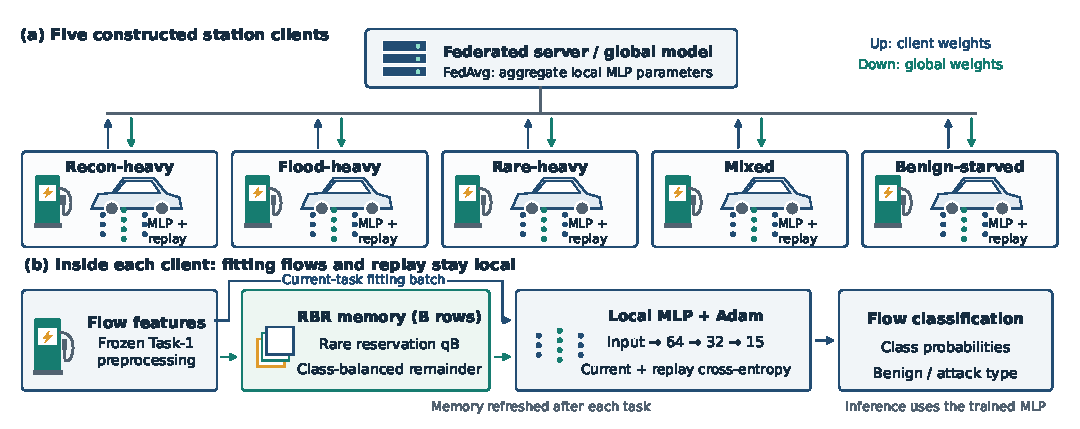
\includegraphics[width=\textwidth]{figures/evse_architecture.pdf}
\caption{EVSE-oriented system architecture. (a) Five constructed client profiles exchange MLP parameters with the server. (b) Local current flows and RBR memory feed training; a parameterized MLP performs inference. EVSE/car illustrations identify the application context; evaluation uses offline network-flow records.}
\label{fig:architecture}
\end{figure*}

\subsection{Tasks and client profiles}
The MLP predicts benign and 14 attack types. Four cohorts are reconnaissance $R$ (aggressive, OS fingerprinting, SYN stealth, service-version and TCP-port scans), flooding $F$ (SYN, TCP, UDP, ICMP, PSHACK and synonymous-IP floods), low-rate/rare $L$ (Slowloris and ICMP fragmentation), and vulnerability scan $V$. Orders are $(R,F,L,V)$, $(F,R,V,L)$ and $(L,V,F,R)$. Benign fitting flows recur in each task. Unseen outputs are masked until their classes arrive.

Five constructed profiles emphasize reconnaissance, flooding or rare traffic, or are mixed or benign-starved. Label-dependent weights, floors and largest-remainder redistribution assign each row to one client; full weights are provided in the supporting tables and repository. The global model is evaluated on each client's held-out flows.


\subsection{Rare-reserved balanced replay}
Let $D_{kt}$ be client $k$'s current fitting rows, $M_{k,t-1}$ its retained memory, $B$ capacity and $\mathcal G=\{\text{Slowloris},\text{ICMP fragmentation}\}$. At the end of task $t$, Algorithm~1 forms unique candidates $C=M_{k,t-1}\cup D_{kt}$ and reserves at most $\lfloor qB\rfloor$ rare candidates. The balanced remainder includes benign and rare classes, so $q$ is a minimum reservation rather than an upper bound. Both stages shuffle each class bucket and cycle through original labels, redistributing unused quota. Thus $|M_{kt}|=\min(B,|C|)$ with no duplicated rows. Discarded attacks are unavailable unless reobserved; benign fitting references recur.

\noindent\begin{minipage}{\columnwidth}
\smallskip\hrule\smallskip
\footnotesize\textbf{Algorithm 1. RBR local memory allocation}\par
\textit{Inputs:} prior memory $M$, current fitting rows $D$, $B,q,\mathcal G$.
\begin{tabular}{@{}r@{\quad}p{0.90\columnwidth}@{}}
1 & $C\leftarrow\operatorname{unique}(M\cup D)$; $C^{\mathcal G}\leftarrow\{i\in C:y_i\in\mathcal G\}$.\\
2 & $a\leftarrow\min(\lfloor qB\rfloor,|C^{\mathcal G}|)$.\\
3 & $A\leftarrow\operatorname{Bal}(C^{\mathcal G},a)$.\\
4 & $M'\leftarrow A\cup\operatorname{Bal}(C\setminus A,B-|A|)$; return $M'$.\\
\end{tabular}
\textit{Bal$(S,b)$:} shuffle buckets by original class; repeatedly take one per nonempty class in sorted-label order until $b$ rows or exhaustion.
\smallskip\hrule\smallskip
\end{minipage}

\subsection{Federated continual optimization}
Algorithm~2 trains on current flows with the memory retained from the previous task, then updates memory for the next task. With replay fraction $r$, local batches minimize
\begin{equation}
\mathcal L_k=(1-r)\operatorname{CE}(D_{kt})+r\operatorname{CE}(M_{k,t-1}).
\label{eq:loss}
\end{equation}
Replay is sampled uniformly with replacement; with empty memory, current-task cross-entropy is used alone. Weighted averaging uses $n_k=|D_{kt}\cup M_{k,t-1}|$ distinct fitting rows:
\begin{equation}
\theta^{s+1}=\sum_{k=1}^{5}\frac{n_k}{\sum_j n_j}\theta_k^{s+1}.
\label{eq:fedavg}
\end{equation}
The pooled centralized control receives $5B$ memory rows, matching total storage. Allocation uses fitting data only, adding no communication beyond model updates.

\noindent\begin{minipage}{\columnwidth}
\smallskip\hrule\smallskip
\footnotesize\textbf{Algorithm 2. Federated continual training with RBR}\par
\textit{Initialize:} global parameters $\theta$; $M_{k0}=\varnothing$ for all clients.
\begin{tabular}{@{}r@{\quad}p{0.90\columnwidth}@{}}
1 & For each task $t$: expose current classes and fitting rows $D_{kt}$.\\
2 & For each of five rounds: broadcast $\theta$ to every client.\\
3 & Each client runs Adam for five local epochs on (\ref{eq:loss}).\\
4 & Aggregate returned parameters using (\ref{eq:fedavg}).\\
5 & After the rounds: score the held-out checkpoint.\\
6 & For each client: $M_{kt}\leftarrow\operatorname{RBR}(M_{k,t-1},D_{kt},B,q,\mathcal G)$.\\
\end{tabular}
\smallskip\hrule\smallskip
\end{minipage}

\section{Experimental Protocol}
We cap each attack type at 3,000 available flows. The fixed sample has 36,172 rows: 23,513 fitting, 5,425 calibration and 7,234 evaluation. Persistent roles are stratified within client/type blocks using target fractions 0.65/0.15/0.20. Preprocessing excludes provenance, addresses, identifiers, absolute timestamps and fingerprint-like fields; scaling and categorical vocabularies fit only Task-1 fitting rows and then freeze. The backbone is input--64--32--15, ReLU and Adam, with five local epochs per round, five rounds per task, batch 128, weight decay $10^{-4}$ and no gradient clipping.

\subsection{Comparators and calibration}
The replay comparison varies memory allocation under a fixed replay loss. EWC, A-GEM and DER++ modify regularization, gradients or replay targets; their mechanisms are complementary and could be combined with the allocation rule. EWC, A-GEM and joint fitting results are retained in the supporting results.

Uniform replay samples candidates randomly; class-balanced applies $\operatorname{Bal}$ to the whole pool. Protected reserves 20\% each for benign and the rare group, then fills randomly. RBR calibrates $q\in\{0.10,0.20\}$; replay methods calibrate $r\in\{0.25,0.50\}$ at learning rate 0.003. Choices maximize mean-checkpoint original-type calibration macro recall, separately for each environment/order/capacity. Fine-tuning and joint calibrate learning rate in $\{0.001,0.003\}$; EWC calibrates $\lambda\in\{1,100\}$ and A-GEM reference batch size in $\{32,64\}$.

CBRS uses the published population rule~\cite{cbrs}: once memory is filled, non-full classes replace a random member of a largest class, while full classes use within-class reservoir replacement with probability $m_c/n_c$. A class remains full after becoming largest in filled memory. Each fitting flow enters the population stream once, counters persist, and population updates occur at the shared task boundary. CBRS calibrates only $r$ on original split 42, at $B=60$, under the same backbone and replay loss. All settings are selected before evaluation; this isolates the CBRS population rule under uniform retrieval, rather than its separate weighted-replay recipe.

\subsection{Scoring}
Primary scoring sums six scan probabilities into one Scan output: the five reconnaissance types and vulnerability scan. Slowloris remains separate; original type labels and task cohorts are retained for training. A scan-only Random Forest fits perfectly but reaches 34.25\% evaluation accuracy, motivating merged scoring. Task-1 categorical vocabularies vary by order, so order comparisons mix representation and sequence effects.

Old accuracy averages final attack accuracy over the first three original cohorts. Forgetting averages each cohort's maximum post-learning accuracy minus its final accuracy. Slowloris recall uses its 600 evaluation flows. Worst-client score is the minimum supported-class macro recall. We report means and sample SD over ten training-seed averages of three orders; paired 95\% $t_9$ intervals use the ten seed differences. Additional role-split seeds 43--45 preserve the sample, allocation and settings, refit Task-1 preprocessing, and recalibrate the key RBR/class-balanced comparison at $B=60$.

\section{Results}
\begin{table}[t]
\centering
\caption{Federated memory 60/client, original split 42. Merged-Scan scores (\%); mean $\pm$ SD of ten seed averages over three orders. Worst is client macro recall.}
\label{tab:main}
\footnotesize
\setlength{\tabcolsep}{2.5pt}
\begin{tabular}{lrrrr}
\toprule
Method & Old acc. $\uparrow$ & Forget $\downarrow$ & Slowloris $\uparrow$ & Worst $\uparrow$\\
\midrule
No replay & 22.22 $\pm$ 0.00 & 77.60 $\pm$ 0.02 & 33.33 $\pm$ 0.00 & 14.81 $\pm$ 0.00\\
Uniform & 65.29 $\pm$ 2.92 & 34.53 $\pm$ 2.93 & 66.98 $\pm$ 7.02 & 45.50 $\pm$ 2.86\\
Class-balanced & 83.99 $\pm$ 1.44 & 15.77 $\pm$ 1.42 & 71.56 $\pm$ 4.19 & 77.97 $\pm$ 1.05\\
CBRS & 83.88 $\pm$ 1.12 & 15.89 $\pm$ 1.12 & 72.57 $\pm$ 2.04 & 77.87 $\pm$ 1.50\\
Protected & 72.84 $\pm$ 2.25 & 26.84 $\pm$ 2.29 & 82.73 $\pm$ 2.36 & 47.15 $\pm$ 3.82\\
\textbf{RBR} & 85.52 $\pm$ 1.27 & 14.24 $\pm$ 1.27 & 76.62 $\pm$ 4.16 & 79.03 $\pm$ 1.00\\
EWC & 24.89 $\pm$ 1.30 & 74.95 $\pm$ 1.30 & 33.33 $\pm$ 0.00 & 17.15 $\pm$ 3.56\\
A-GEM & 46.03 $\pm$ 4.58 & 53.80 $\pm$ 4.58 & 50.29 $\pm$ 4.68 & 37.12 $\pm$ 3.29\\
Joint & 94.20 $\pm$ 0.07 & -- & 76.82 $\pm$ 0.17 & 77.89 $\pm$ 1.48\\
\bottomrule
\end{tabular}
\end{table}


\subsection{Retention and Slowloris at memory 60}
Table~\ref{tab:main} summarizes the primary comparison. RBR reaches 85.52\% old accuracy and 76.62\% Slowloris recall. Over class-balanced, gains are $+1.53$ points $[0.23,2.84]$ for old accuracy and $+5.06$ $[1.27,8.84]$ for Slowloris; forgetting falls by 1.54 points. Worst-client difference is $+1.06$ $[-0.07,2.19]$. Exact-type scores are retained in the supporting results.

Against protected, RBR gains 12.68 points of old accuracy and 31.87 of worst-client score, while losing 6.11 points of Slowloris. The rare+random/no-benign ablation reaches 72.07\% old accuracy, 84.78\% Slowloris and 48.62\% worst-client score: RBR changes these by $+13.45$, $-8.16$ and $+30.41$ points, respectively, with all three paired intervals excluding zero. This exposes the retention--Slowloris trade-off of random filling.

Federated RBR minus CBRS differences are old accuracy $+1.64$ $[0.40,2.88]$, Slowloris $+4.04$ $[0.41,7.68]$, and worst-client $+1.16$ $[0.02,2.30]$. Centralized RBR minus CBRS differences are old accuracy $+3.25$ $[2.21,4.30]$, Slowloris $+7.93$ $[4.09,11.77]$, and worst-client $+0.49$ $[-0.68,1.66]$. In centralized order 2, the slowloris recall difference is $-0.58$ $[-1.07,-0.10]$. With exact types, federated old-accuracy and Slowloris differences are $+0.23$ $[-1.75,2.21]$ and $+3.57$ $[-0.92,8.06]$; both intervals include zero.

\subsection{Capacity, split consistency and federation}

At memory 300, RBR improves old accuracy, Slowloris and worst-client score over class-balanced by 1.68, 5.94 and 0.42 points, respectively; each interval excludes zero. Protected exceeds RBR on old accuracy and Slowloris by 1.30 and 5.08 points, while RBR retains a 6.19-point worst-client advantage.
\begin{figure}[t]
\centering
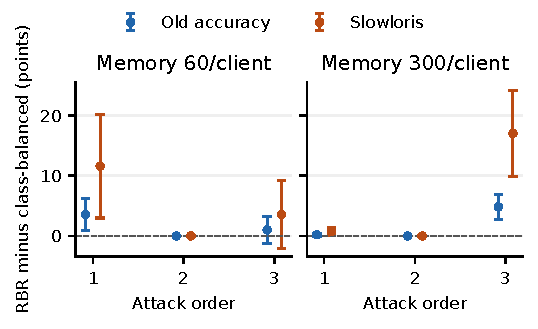
\includegraphics[width=\columnwidth]{figures/order_effects.pdf}
\caption{RBR minus class-balanced by order and capacity, original split. Bars are paired 95\% intervals over ten seeds.}
\label{fig:orders}
\end{figure}
Fig.~\ref{fig:orders} shows order variation. At memory 60, Slowloris gains are 11.60, 0 and 3.57 points across the three orders; order 2 ends with the rare cohort, where both methods reach full recall. At memory 300, RBR loses old accuracy to protected in orders 1 and 2.

The gains hold under federated heterogeneity and align with centralized controls at matched total storage. Centralized RBR gains over class-balanced at memory 60 are 1.67 points of old accuracy and 5.00 of Slowloris. Federated-minus-centralized differences in improvement are $-0.14$ $[-1.54,1.26]$ and $+0.06$ $[-4.26,4.38]$, respectively. Retention and Slowloris differences are positive on all four splits in both settings; both federated gains are significant on each split (Table~\ref{tab:fedsplits}). Centralized significance varies across splits. The rare-heavy/benign-starved profiles have RBR macro recall 79.25/88.55\%, versus 78.30/88.58\% with class-balanced replay.


\begin{table}[t]
\centering
\caption{Federated RBR minus class-balanced, $B=60$: percentage points [95\% paired interval], all four splits.}
\label{tab:fedsplits}
\footnotesize
\setlength{\tabcolsep}{3pt}
\begin{tabular}{llrr}
\toprule
Split & Setting & Old accuracy & Slowloris\\
\midrule
42 & Fed. & $+1.53$ $[0.23,2.84]$ & $+5.06$ $[1.27,8.84]$\\
43 & Fed. & $+2.23$ $[0.95,3.51]$ & $+7.93$ $[4.03,11.83]$\\
44 & Fed. & $+3.37$ $[2.11,4.63]$ & $+11.28$ $[7.59,14.97]$\\
45 & Fed. & $+2.06$ $[0.40,3.72]$ & $+6.09$ $[1.30,10.88]$\\
\bottomrule
\end{tabular}
\end{table}

\section{Conclusion}
RBR improves retention and Slowloris recognition over class-balanced replay across the tested federated splits. Its balanced remainder preserves broader class coverage than random filling, while rare reservation improves Slowloris recall. Against CBRS, the primary merged-Scan results support an average improvement at memory 60, with order-specific and exact-type differences reported above. Matched centralized controls show that these gains remain useful under the tested federated heterogeneity.

\textit{Limitations:} Validation uses one dataset and constructed, row-split clients; benign/fragmentation support is insufficient for corresponding claims. EWC tuning is limited; intervals are unadjusted.

\noindent\textbf{Code and data availability.} Code, configurations and split manifests: \url{https://github.com/f20230006-sketch/evse-fcl-multiclass-pilot} (private repository; access required). Dataset source:~\cite{dataset}.

\IEEEtriggeratref{4}
\begin{thebibliography}{18}
\bibitem{ocpp} Z. Garofalaki, D. Kosmanos, S. Moschoyiannis, D. Kallergis, and C. Douligeris, ``Electric vehicle charging: A survey on the security issues and challenges of the Open Charge Point Protocol (OCPP),'' arXiv:2207.01950, 2022, doi: 10.1109/COMST.2022.3184448.
\bibitem{dataset} Canadian Institute for Cybersecurity, ``CIC EV charger attack dataset 2024 (CICEVSE2024),'' University of New Brunswick, 2024. [Online]. Available: \url{https://www.unb.ca/cic/datasets/evse-dataset-2024.html}
\bibitem{slowloris} R. Giobbi, ``Mitigating Slowloris,'' 2009. [Online]. Available: \url{https://www.sei.cmu.edu/blog/mitigating-slowloris/}
\bibitem{diot} T. D. Nguyen \emph{et al.}, ``D-IoT: A federated self-learning anomaly detection system for IoT,'' in \emph{Proc. IEEE ICDCS}, pp. 756--767, 2019, doi: 10.1109/ICDCS.2019.00080.
\bibitem{kitsune} Y. Mirsky, T. Doitshman, Y. Elovici, and A. Shabtai, ``Kitsune: An ensemble of autoencoders for online network intrusion detection,'' in \emph{Proc. NDSS}, 2018, doi: 10.14722/ndss.2018.23204.
\bibitem{amr} S. K. Amalapuram, S. S. Channappayya, and B. R. Tamma, ``Augmented memory replay-based continual learning approaches for network intrusion detection,'' in \emph{Advances in Neural Information Processing Systems}, vol. 36, 2023.
\bibitem{fedavg} B. McMahan, E. Moore, D. Ramage, S. Hampson, and B. A. y Arcas, ``Communication-efficient learning of deep networks from decentralized data,'' in \emph{Proc. AISTATS}, PMLR, vol. 54, pp. 1273--1282, 2017.
\bibitem{fedprox} T. Li \emph{et al.}, ``Federated optimization in heterogeneous networks,'' in \emph{Proc. MLSys}, vol. 2, 2020.
\bibitem{scaffold} S. P. Karimireddy \emph{et al.}, ``SCAFFOLD: Stochastic controlled averaging for federated learning,'' in \emph{Proc. ICML}, PMLR, vol. 119, pp. 5132--5143, 2020.
\bibitem{fedweit} J. Yoon, W. Jeong, G. Lee, E. Yang, and S. J. Hwang, ``Federated continual learning with weighted inter-client transfer,'' in \emph{Proc. ICML}, 2021, arXiv:2003.03196.
\bibitem{tiny} A. Chaudhry \emph{et al.}, ``On tiny episodic memories in continual learning,'' arXiv:1902.10486, 2019.
\bibitem{icarl} S.-A. Rebuffi, A. Kolesnikov, G. Sperl, and C. H. Lampert, ``iCaRL: Incremental classifier and representation learning,'' in \emph{Proc. CVPR}, pp. 2001--2010, 2017.
\bibitem{gem} D. Lopez-Paz and M. Ranzato, ``Gradient episodic memory for continual learning,'' in \emph{Advances in Neural Information Processing Systems}, vol. 30, 2017.
\bibitem{agem} A. Chaudhry, M. Ranzato, M. Rohrbach, and M. Elhoseiny, ``Efficient lifelong learning with A-GEM,'' in \emph{Proc. ICLR}, 2019.

\bibitem{ewc} J. Kirkpatrick \emph{et al.}, ``Overcoming catastrophic forgetting in neural networks,'' \emph{Proc. Natl. Acad. Sci. USA}, vol. 114, no. 13, pp. 3521--3526, 2017, doi: 10.1073/pnas.1611835114.
\bibitem{der} P. Buzzega, M. Boschini, A. Porrello, D. Abati, and S. Calderara, ``Dark experience for general continual learning: A strong, simple baseline,'' in \emph{Advances in Neural Information Processing Systems}, vol. 33, 2020.
\bibitem{cbrs} A. Chrysakis and M.-F. Moens, ``Online continual learning from imbalanced data,'' in \emph{Proc. ICML}, PMLR, vol. 119, pp. 1952--1961, 2020.
\bibitem{fedcbdr} Z. Qi, Y.-P. Tang, L. Meng, H. Yu, X. Li, and X. Meng, ``Class-wise balancing data replay for federated class-incremental learning,'' arXiv:2507.07712, 2025.
\end{thebibliography}

\end{document}
